% ---------------------------------------------------
% ----- Main document of the template
% ----- for Bachelor-, Master thesis and class papers
% ---------------------------------------------------
%  Created by C. Müller-Birn on 2012-08-17, CC-BY-SA 3.0.
%  Last upadte: C. Müller-Birn 2015-11-27
%  Freie Universität Berlin, Institute of Computer Science, Human Centered Computing. 

\documentclass[pdftex,a4paper,12pt,DIV=calc,BCOR5mm,ngerman,twoside,smallheadings,titlepage]{scrbook}   
% ----- weitere Optionen 
%draft,			% Entwurfsmodus zum Anzeigen zu leerer/voller Boxen 
%DIV=calc
%DIV12,			% Seitengröße (siehe Koma Skript Dokumentation !) 
%BCOR5mm,		% Zusätzlicher Rand auf der Innenseite 
%twoside,		% Seitenränder werden an doppelseitig angepasst 
%fleqn,			% Formeln werden linksbündig (und nicht zentriert) angezeigt 
%titlepage,		% Titel wird in einer 'titlepage' Umgebung gesetzt 
%bigheadings,	% Große Überschriften (normal, small-headings) 
%halfparskip-	% Absatz wird nicht eingerückt, dafür aber um eine halbe Zeile nach unten gerückt
%
%---------------------------------------------------
%----- Packages
%---------------------------------------------------
%
\usepackage[T1]{fontenc} 
\usepackage[utf8]{inputenc}
\usepackage[ngerman]{babel} %\usepackage[english]{babel}  
\usepackage{ae} 
\usepackage{bibgerm}    

\usepackage{fancyhdr} % Define simple headings 
\usepackage{xcolor}
\usepackage{url}
\usepackage{listings}
%\usepackage{vmargin} % Adjust margins in a simple way
%
\usepackage{amsmath}
%
\usepackage[pdftex]{graphicx}  
\usepackage{hyperref} % turn all your internal references into hyperlinks
%\usepackage[pdfstartview=FitH,pdftitle={<<Titel der Arbeit>>}, pdfauthor={<<Autor>>}, pdfkeywords={<<Schlüsselwörter>>}, pdfsubject={<<Titel der Arbeit>>}, colorlinks=true, linkcolor=black, citecolor=black, urlcolor=black, hypertexnames=false, bookmarksnumbered=true, bookmarksopen=true, pdfborder = {0 0 0}]{hyperref}
%
% table settings 
\usepackage{booktabs}  
\usepackage{tabularx}  
\usepackage{rotating}
\usepackage{longtable}
\usepackage{pdflscape}
\usepackage{multirow} %multi row
\usepackage{rotating} %for rotating table
%
%---------------------------------------------------
%----- PDF and document setup
%---------------------------------------------------
%
\hypersetup{
	pdftitle={<My title>},  % please, add the title of your thesis
    pdfauthor={<Author>},   % please, add your name
    pdfsubject={<<Bachelor/Master thesis>, Institute of Computer Science, Freie Universität Berlin>}, % please, select the type of this document
    pdfstartview={FitH},    % fits the width of the page to the window
    pdfnewwindow=true, 		% links in new window
    colorlinks=false,  		% false: boxed links; true: colored links
    linkcolor=red,          % color of internal links
    citecolor=green,        % color of links to bibliography
    filecolor=magenta,      % color of file links
    urlcolor=cyan           % color of external links
}
% 
%---------------------------------------------------
%----- Customize page size
%---------------------------------------------------
\usepackage[top=3cm,right=3cm,bottom=4cm,left=4cm]{geometry}    
%
%---------------------------------------------------
%----- Customize header and footer\pagestyle{fancy} 
%---------------------------------------------------
\pagestyle{fancy}

\fancyhf{}  % delete all existing header formating

\fancyhead[LE]{\leftmark}  % represent the current chapter heading in uppercase
\renewcommand{\chaptermark}[1]{ % adapt the shown chapter name: show it in lower case and with chapter number 
\markboth{\thechapter.\ #1}{}}   

\fancyhead[RO]{\rightmark}   % % represent the current section heading in uppercase 
\renewcommand{\sectionmark}[1]{% adapt the shown section name: show it in lower case and with section number 
\markboth{\thesection.\ #1}{}}

\renewcommand{\headrulewidth}{0pt} % remove lines from header
\renewcommand{\footrulewidth}{0pt} % remove lines from header

\fancyfoot{} % delete all existing footer formating
\fancyfoot[LE,RO]{\thepage} % put page number on the left on even page and right on odd page
%
%---------------------------------------------------      
%----- Settings for word separation  
%---------------------------------------------------      
% Help for separation (from package babel, section 22)):
% In german package the following hints are additionally available:
% "- = an explicit hyphen sign, allowing hyphenation in the rest of the word
% "| = disable ligature at this position. (e.g., Schaf"|fell)
% "~ = for a compound word mark without a breakpoint (e.g., bergauf und "~ab)
% "= = for a compound word mark with a breakpoint, allowing hyphenation in the composing words
% "" = like "-, but producing no hyphen sign (e.g., und/""oder)
%
% Describe separation hints here:
\hyphenation{
% Pro-to-koll-in-stan-zen
% Ma-na-ge-ment  Netz-werk-ele-men-ten
% Netz-werk Netz-werk-re-ser-vie-rung
% Netz-werk-adap-ter Fein-ju-stier-ung
% Da-ten-strom-spe-zi-fi-ka-tion Pa-ket-rumpf
% Kon-troll-in-stanz
}
%
%---------------------------------------------------
%----- Restricting including files   
%---------------------------------------------------
% Only files listed here will be included in the PDF document!
% In order to only partially translate the document, for example for bug-fixing, 
% it might be useful to comment out some of the documents.
\includeonly{
title,
declaration,
abstract_en,
abstract_de,
preface,
introduction,
chapters,
conclusion,
appendix
}

%%%%%%%%%%%%%%%%%%%%%%%%%%%%%%%%%%%%%%%%%%%%%%%%%%%%%%
% The content part of the documentent starts here! %%
%%%%%%%%%%%%%%%%%%%%%%%%%%%%%%%%%%%%%%%%%%%%%%%%%%%%%%

\begin{document}
%---------------------------------------------------
%----- Listing and color definition   
%---------------------------------------------------
\definecolor{red}{rgb}{.8,.1,.2}
\definecolor{blue}{rgb}{.2,.3,.7}
\definecolor{lightyellow}{rgb}{1.,1.,.97}
\definecolor{gray}{rgb}{.7,.7,.7}
\definecolor{darkgreen}{rgb}{0,.5,.1}
\definecolor{darkyellow}{rgb}{1.,.7,.3}
\lstloadlanguages{C++,[Objective]C}
\lstset{
		escapeinside={§§}{§§},
        basicstyle=\ttfamily\footnotesize\mdseries,
        columns=fullflexible,% typewriter font look better with fullflex
        keywordstyle=\bfseries\color{blue},
%		identifierstyle=\bfseries,
        commentstyle=\color{darkgreen},      
        stringstyle=\color{red},
        numbers=left,
        numberstyle=\ttfamily\scriptsize\color{gray},
%       stepnumber=5,
%       numberfirstline=true,
        breaklines=true,
%		prebreak=\\,
        showstringspaces=true,
        tabsize=4,
        captionpos=b,
%		framexrightmargin=-.2\textwidth,
        float=htb,
		frame=tb,
		frameshape={RYR}{n}{n}{RYR},
		rulecolor=\color{darkyellow},
        xleftmargin=15pt,
        xrightmargin=4pt,
        aboveskip=\bigskipamount,
        belowskip=\bigskipamount,
		backgroundcolor=\color{lightyellow},
		extendedchars=true,
       	belowcaptionskip=15pt
}

%---------------------------------------------------
%----- Title and declaration   
%---------------------------------------------------
\pagenumbering{alph} % even though, these page numbers are not visible there are necessary to have unique page numbers 
% ---------------------------------------------------
% ----- Title page of the template
% ----- for Bachelor-, Master thesis and class papers
% ---------------------------------------------------
%  Created by C. Müller-Birn on 2012-08-17, CC-BY-SA 3.0.
%  Freie Universität Berlin, Institute of Computer Science, Human Centered Computing. 
%
\begin{titlepage}

\title{
{\small Bachelorarbeit am Institut für Informatik der Freien Universität Berlin}\\
{\small Human-Centered Computing (HCC)}\\
[6ex]
{\LARGE Interactive Visualization Interface of Text Exploration and Annotation}}

\author{
{\emph{\normalsize Daniel Stachnik}}\\
{\normalsize Matrikelnummer: 5001807}\\
{\normalsize danstach@zedat.fu-berlin.de}\\ 
[18ex]   
{\normalsize Betreuerin und Erstgutachterin: Prof. Dr. C. Müller-Birn} \\
{\normalsize Zweitgutachter: Prof. Dr. E. Ntoutsi}}
\vspace{6ex}
\date{\normalsize Berlin, 17.07.2021}

\maketitle

\end{titlepage}
% ---------------------------------------------------
% ----- Declaration of the template
% ----- for Bachelor-, Master thesis and class papers
% ---------------------------------------------------
%  Created by C. Müller-Birn on 2012-08-17, CC-BY-SA 3.0.
%  Freie Universität Berlin, Institute of Computer Science, Human Centered Computing. 
%
\pagestyle{empty}

\subsection*{Eidesstattliche Erklärung}

Ich versichere hiermit an Eides Statt, dass diese Arbeit von niemand anderem als meiner Person verfasst worden ist. Alle verwendeten Hilfsmittel wie Berichte, Bücher, Internetseiten oder ähnliches sind im Literaturverzeichnis angegeben, Zitate aus fremden Arbeiten sind als solche kenntlich gemacht. Die Arbeit wurde bisher in gleicher oder ähnlicher Form keiner anderen Prüfungskommission vorgelegt und auch nicht veröffentlicht.
\par\bigskip  
\noindent Berlin, den \today

\vspace{1.2cm}

\noindent Daniel Stachnik  

\cleardoublepage

%---------------------------------------------------
%----- Abstracts in English and German   
%---------------------------------------------------

% ---------------------------------------------------
% ----- Abstract (English) of the template
% ----- for Bachelor-, Master thesis and class papers
% ---------------------------------------------------
%  Created by C. Müller-Birn on 2012-08-17, CC-BY-SA 3.0.
%  Freie Universität Berlin, Institute of Computer Science, Human Centered Computing. 
%
\pagestyle{empty}

\subsection*{Abstract}

<Please summarize your thesis in a brief but meaningful way (about one page). Include in your abstract the topic of this thesis, important contents, results of your research and an evaluation of your results.> Explainable artificial intelligence has become a topic of big interest in research. 

\cleardoublepage

% ---------------------------------------------------
% ----- Abstract (German) of the template
% ----- for Bachelor-, Master thesis and class papers
% ---------------------------------------------------
%  Created by C. Müller-Birn on 2012-08-17, CC-BY-SA 3.0.
%  Freie Universität Berlin, Institute of Computer Science, Human Centered Computing. 
%
\pagestyle{empty}

\subsection*{Zusammenfassung}

<Hier sollten Sie eine kurze, aussagekräftige Zusammenfassung (ca. eine Seite) Ihrer Arbeit geben, welche das Thema der Arbeit, die wichtigsten Inhalte, die Arbeitsergebnisse und die Bewertung der Ergebnisse umfasst.> 

\cleardoublepage  
                                          
%---------------------------------------------------
%----- Directories   
%---------------------------------------------------

\frontmatter 
\pagenumbering{roman}

\tableofcontents
\setcounter{tocdepth}{3}   % reduce the included sections in the table of content

\listoffigures
\listoftables

%---------------------------------------------------
%----- Main part
%---------------------------------------------------
\mainmatter
\pagenumbering{arabic} 
\pagestyle{fancy} 

% ---------------------------------------------------
% ----- Preface of the template
% ----- for Bachelor-, Master thesis and class papers
% ---------------------------------------------------
%  Created by C. Müller-Birn on 2012-08-17, CC-BY-SA 3.0.
%  Freie Universität Berlin, Institute of Computer Science, Human Centered Computing. 
%
\chapter*{Vorwort}
\label{chap:preface}

\section*{Allgemeine Hinweise zur Erstellung einer Abschlussarbeit}

\begin{itemize}
	\item Beachten Sie, dass diese Vorlage für einen zweiseitigen Ausdruck angelegt wurde.  
	\item Über die Papierqualität können Sie entscheiden, aber wir empfehlen aber Seiten mit wichtigen, farbigen Grafiken auch in Farbe auszudrucken und dabei ein höherwertiges Papier zu verwenden. 
	\item Bitte stimmen Sie mit dem Betreuer Ihrer Arbeit auch den Zweitgutachter ab. Die Anfrage des Zweitgutachters erfolgt von Ihnen. Es ist an dieser Stelle sinnvoll, die Anfrage mit einer kurzen Zusammenfassung der Arbeit zu stellen.  
	\item Bitte beachten Sie, dass Sie Ihre Abschlussarbeit mit einer Klebebindung versehen, eine Ringbindung ist nicht erwünscht. 
\end{itemize} 

% ---------------------------------------------------
% ----- Introduction of the template
% ----- for Bachelor-, Master thesis and class papers
% ---------------------------------------------------
%  Created by C. Müller-Birn on 2012-08-17, CC-BY-SA 3.0.
%  Last upadte: C. Müller-Birn 2015-11-27 
%  Freie Universität Berlin, Institute of Computer Science, Human Centered Computing. 
%
\chapter{Einleitung}
\label{chap:introduction}

Im folgenden werden Ihnen Hinweise zur Strukturierung und zum Inhalt des ersten Kapitels gegeben.

\section{Thema und Kontext}
\begin{itemize}
	\item Wo setze ich an? (Problemstellung / Ausgangslage)      
	\item Identifikation der signifikanten Problemen im betrachteten Forschungsbereich  
	\item Ein kurzer Überblick über den aktuellen Forschungsstand in dem Bereich inklusive vorhandener Lösungen (ausführlicher dann in den Folgeabschnitten)
\end{itemize}

\section{Zielsetzung der Arbeit}
\begin{itemize}
	\item Was sind die mit dieser Arbeit verfolgten Ziele? Welches Problem soll gelöst werden?
	\item Eine Beschreibung der ersten Ideen, der vorgeschlagene Ansatz und die aktuell erreichten Resultate 
	\item Eine Beschreibung, welchen Beitrag die Arbeit leistet, um das vorgestellte Problem zu lösen
	\item Eine Diskussion, wie die vorgeschlagene Lösung sich von bestehenden unterscheidet, was ist neu oder besser?
\end{itemize}

\section{Vorgehen bei der Umsetzung}
\begin{itemize}
	\item Wie will ich meine Ziele erreichen? (Methodische Überlegungen)
	\item Darstellung zum Forschungsdesign.
	\item Insbesondere bei Master: Wie kann die Zielerreichung ``gemessen'' werden? 
\end{itemize}  	

\section{Aufbau der Arbeit}
\begin{itemize}
	\item Welche Schritte werden durchlaufen, um die Ziele zu erreichen?
	\item An dieser Stelle ist beispielsweise eine Grafik hilfreich, um den Aufbau der Arbeit und welche Ergebnisse/Erkenntnisse wo genutzt werden, zu visualisieren. 
	\item Ebenfalls sollten noch Anmerkungen zur Gestaltung der Arbeit gegeben werden, vor allem, da in vielen deutschen Arbeiten englische Fachbegriffe verwendet werden. Ein solcher Text könnte folgendermaßen lauten: 
		\begin{itemize}
			\item ``Abschließend sind hier noch eine Anmerkungen zur Gestaltung der vorliegenden Arbeit. Für die im Folgenden verwendeten personenbezogene Ausdrücke wurde, um die Lesbarkeit der Arbeit zu erhöhen, die männliche Schreibweise gewählt. Des Weiteren werden eine Reihe von englischen Bezeichnungen verwendet, um einerseits dem interessierten Leser das Studium der häufig vorliegenden englischen Originalliteratur zu erleichtern oder andererseits bestehende Fachbegriffe nicht durch die Übersetzung zu verfälschen. Diese Begriffe sind vom herkömmlichen Text in kursiver Schrift unterschieden.''
		\end{itemize}
\end{itemize}

\begin{figure}[!ht]
	% Mit [!h] wird die Position der Grafik bestimmt. So bedeutet h=here und mit dem "!" (Ausrufezeichen) wird dieser Befehl verstärkt. Weitere Möglichkeiten sind : t=top und b=bottom. Zumeist wird angegeben, in welcher Reihenfolge LaTeX versuchen soll das Bild einzufügen, z.B. [!htb].
	\centering
		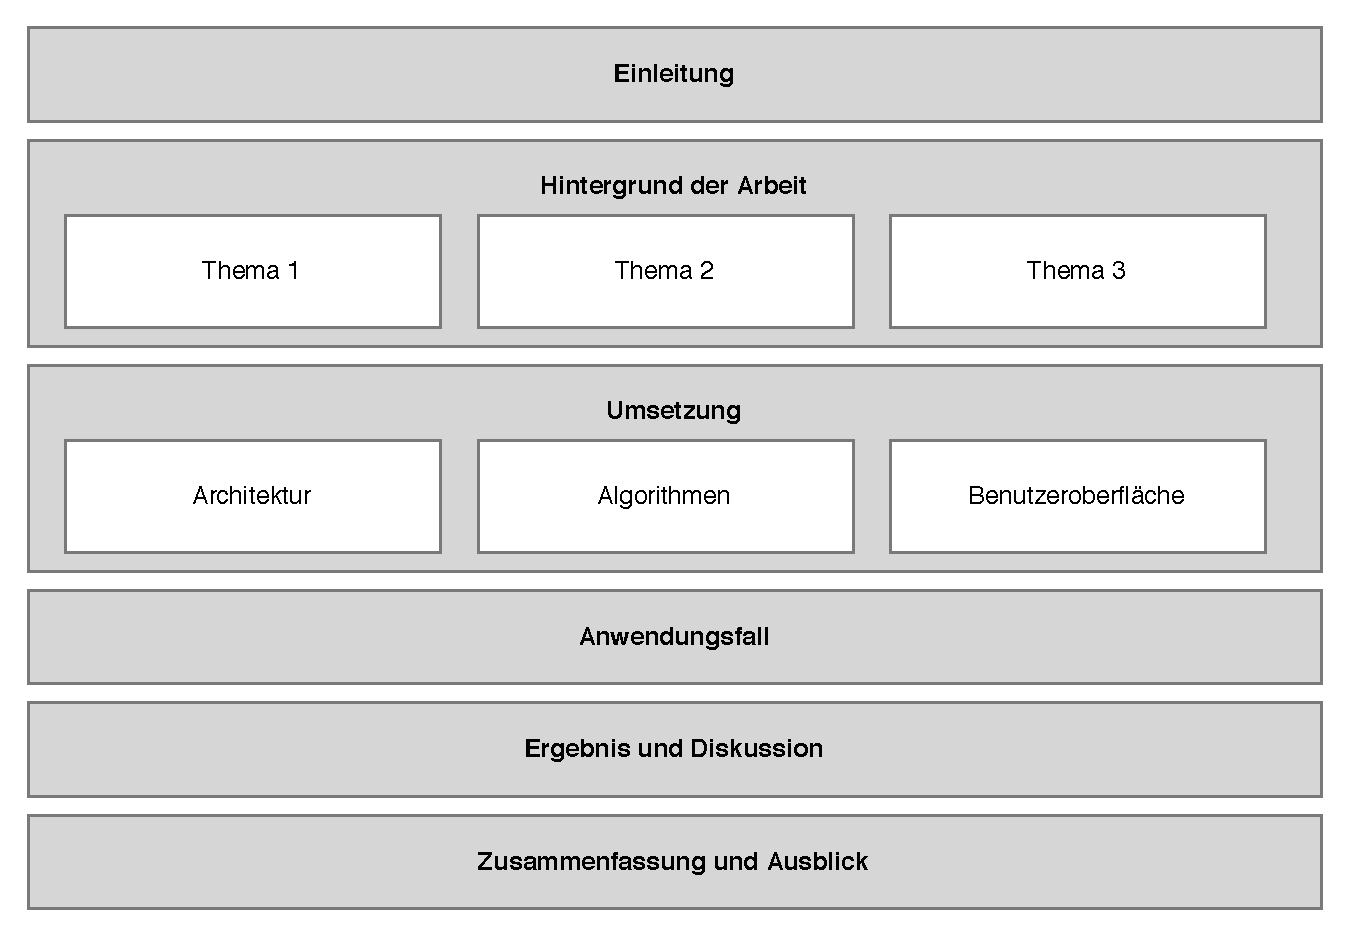
\includegraphics[width=0.95\textwidth]{pics/structure.pdf}
	\caption[Beispiel einer möglichen Darstellung zum Aufbau der Arbeit]{Beispiel einer möglichen Darstellung zum Aufbau der Arbeit (vgl. Beschreibung Abschnitt  \ref{chap:chapters}).} 
	% Mit Hilfe von caption wird die Bildunterschrift erzeugt. Der Text in geschweiften Klammern erscheint im Text, während der Text in eckigen Klammern sich dann empfiehlt, wenn die Beschreibung besonders lang ist, denn diese wird dann im Bildverzeichnis verwendet. Diese Kurzbeschreibung kann auch weggelassen werden. 
	\label{fig:structurethesis}
\end{figure}
% ---------------------------------------------------
% ----- Chapters of the template
% ----- for Bachelor-, Master thesis and class papers
% ---------------------------------------------------
%  Created by C. Müller-Birn on 2012-08-17, CC-BY-SA 3.0.
%  Freie Universität Berlin, Institute of Computer Science, Human Centered Computing. 
%
\chapter{Kapitel}
\label{chap:chapters} 

\begin{itemize}
	\item Abhängig vom Ziel der Arbeit und dem verwendeten Forschungsdesign unterscheidet sich dieser Hauptteil der Arbeit erheblich. 
	\item Eine sehr allgemeine Struktur ist die folgende:
	\begin{itemize}
		\item Hintergrund der Arbeit (Theoretische Einordnung der Arbeit) 
		 	\begin{itemize}
		 		\item Hier sollte enthalten sein, welche Anwendungen in diesem Bereich bereits existieren und warum bei diesen ein Defizit besteht. 
				\item Falls genutzt, sollten hier die entsprechenden Algorithmen erläutert werden.
				\item Es sollten die Ziele der Anwendungsentwicklung, d.h. die Anforderungen herausgearbeitet werden. Dabei sollte die bestehende Literatur geeignet integriert werden.
		 	\end{itemize}
		\item Umsetzung (Praktischer Anteil der Arbeit)
			\begin{itemize}
				\item Zunächst sollte die Softwarearchitektur und die genutzten Anwendungen, APIs etc. erläutert werden. Ebenfalls gehört dazu das Datenbankschema.
				\item Es sollten die zentralen Elemente der Software (abhängig von der Aufgabenstellung) beschrieben werden, wie implementierte Algorithmen oder das Oberflächendesign.
				\item Zentraler Quellcode sollte entsprechend aufgelistet werden:
				\lstset{language=Java,basicstyle=\footnotesize,numbers=left,showstringspaces=false,frame=single}
				\begin{lstlisting}
				public class Main {
					public static void main(String[] args) {
						System.out.println("Hello World!");
					}
				}
				\end{lstlisting} 
				%\item Klassendiagramm für Backend
				%\item Dr Quellcode zentraler Implementierungen  können als Auszug in den Anhang. Im Text kann dann darauf verwiesen werden.
			\end{itemize}
		\item Evaluation (zumeist nur für Masterarbeiten relevant)
		\begin{itemize}
			\item Jede Software muss auch getestet werden. Dieses Tests werden entweder mit einem vorgegebenen Datensatz erfolgen oder aber die Evaluation erfolgt auf Basis von Experimenten. In diesem Kapitel sollte daher entweder der genutzte Datensatz oder der experimentelle Aufbau beschrieben werden. 
		\end{itemize}
		\item Ergebnis und Diskussion
		\begin{itemize}
			\item Die Ergebnisse der Anwendung werden in diesem Kapitel vorgestellt und anschließend diskutiert. Wenn möglich sollte die Ergebnisse in Relation zu bestehenden Arbeiten in dem Bereich erörtert werden.
		\end{itemize}
	\end{itemize}  
\end{itemize}
% ---------------------------------------------------
% ----- Conclusion of the template
% ----- for Bachelor-, Master thesis and class papers
% ---------------------------------------------------
%  Created by C. Müller-Birn on 2012-08-17, CC-BY-SA 3.0.
%  Freie Universität Berlin, Institute of Computer Science, Human Centered Computing. 
%
\chapter{Zusammenfassung und Ausblick}
\label{chap:conclusion}      

\begin{itemize}
	\item Die Zusammenfassung sollte das Ziel der Arbeit und die zentralen Ergebnisse beschreiben. Des Weiteren sollten auch bestehende Probleme bei der Arbeit aufgezählt werden und Vorschläge herausgearbeitet werden, die helfen, diese Probleme zukünftig zu umgehen. Mögliche Erweiterungen für die umgesetzte Anwendung sollten hier auch beschrieben werden.
\end{itemize}


%---------------------------------------------------
%----- Bibliography
%---------------------------------------------------
\phantomsection
\addcontentsline{toc}{chapter}{Literatur}
\bibliographystyle{alpha}
\bibliography{references.bib}


%---------------------------------------------------
%----- Appendix   
%---------------------------------------------------
\backmatter
% ---------------------------------------------------
% ----- Appendix of the template
% ----- for Bachelor-, Master thesis and class papers
% ---------------------------------------------------
%  Created by C. Müller-Birn on 2012-08-17, CC-BY-SA 3.0.
%  Freie Universität Berlin, Institute of Computer Science, Human Centered Computing. 
%

\chapter{Appendix}
\label{ch:Appendix}

\section{Erster Teil Appendix}
\label{app:first_appendix} 

\section{Zweiter Teil Appendix}
\label{app:second_appendix}  



\end{document}